%(BEGIN_QUESTION)
% Copyright 2006, Tony R. Kuphaldt, released under the Creative Commons Attribution License (v 1.0)
% This means you may do almost anything with this work of mine, so long as you give me proper credit

Termoelementledning kan i noen tilfeller være kostbar. Anta at en tekniker vil spare penger og bruker et par kobberledere mellom termoelementhodet og kontrollrommet der indikatoren står, i stedet for termoelementledning eller forlengelsesledning:

$$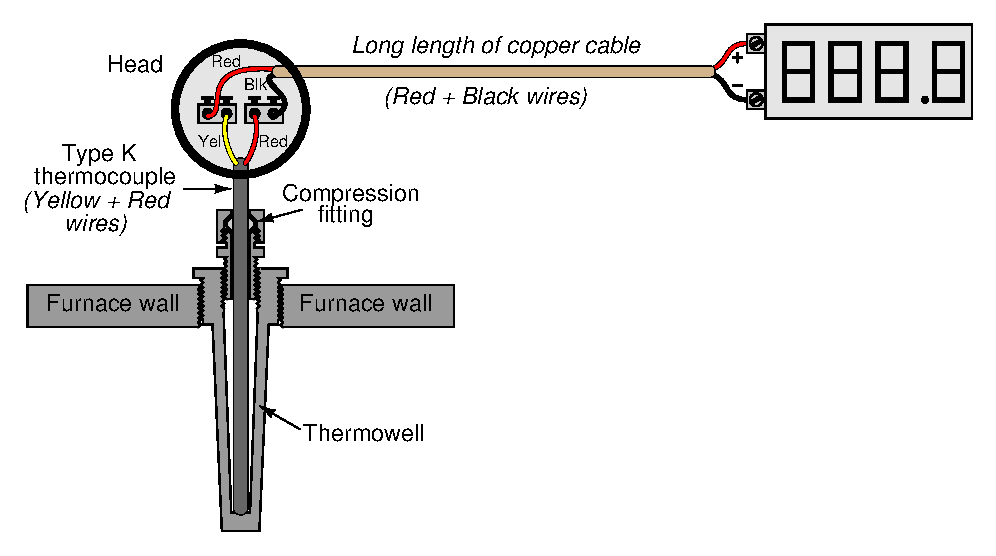
\includegraphics[width=15.5cm]{i00374x01.eps}$$

Tegnet mer som et elektrisk skjema ser kretsen slik ut:

$$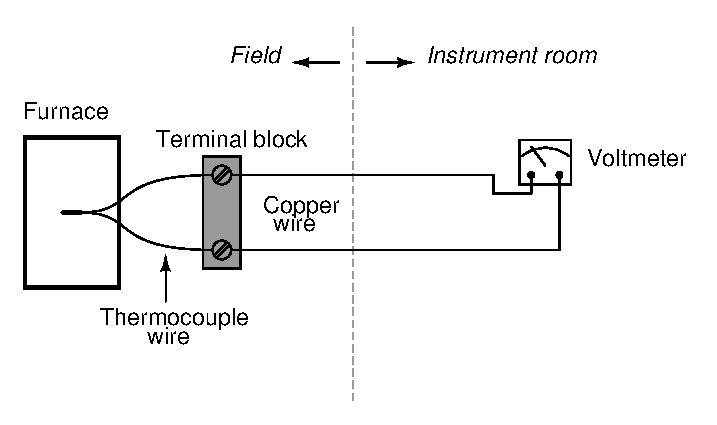
\includegraphics[width=15.5cm]{i00374x02.eps}$$

Forklar hvorfor dette ``sparetipset'' er en dårlig idé.

\underbar{file i00374}
%(END_QUESTION)





%(BEGIN_ANSWER)

Forbindelsene inne i termoelementhodet danner en referanseskjøt. Temperaturen i denne skjøten trekkes fra ovnstemperaturen og bestemmer dermed totalspenningen som indikatoren i kontrollrommet mottar.

%(END_ANSWER)





%(BEGIN_NOTES)


%INDEX% Measurement, temperature: thermocouple

%(END_NOTES)
